\documentclass[tikz]{standalone}
\usetikzlibrary{positioning, fit, backgrounds}

\begin{document}
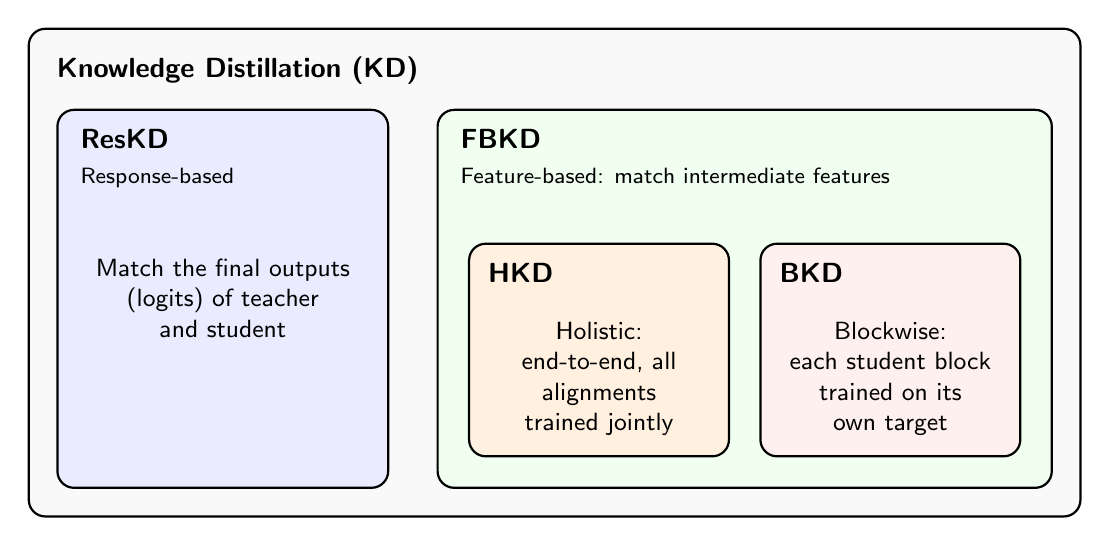
\begin{tikzpicture}[
    every node/.style={font=\sffamily},
    set/.style={draw, thick, rounded corners=6pt, inner sep=0pt},
    title/.style={font=\sffamily\bfseries, anchor=north west, inner sep=0pt},
    sub/.style={font=\sffamily\footnotesize, anchor=north west, inner sep=0pt},
    body/.style={font=\sffamily\small, align=center, anchor=north, inner sep=0pt},
]

% ── Feature-based KD (right region) ─────────────────────────────────────────
\node[set, fill=green!6, minimum width=7.8cm, minimum height=4.8cm] (fbkd) {};
\node[title] at ([shift={(0.3cm,-0.25cm)}]fbkd.north west) {FBKD};
\node[sub]   at ([shift={(0.3cm,-0.75cm)}]fbkd.north west) {Feature-based: match intermediate features};

\node[set, fill=orange!12, minimum width=3.3cm, minimum height=2.7cm, anchor=south west]
      (hkd) at ([shift={(0.4cm,0.4cm)}]fbkd.south west) {};
\node[title] at ([shift={(0.25cm,-0.25cm)}]hkd.north west) {HKD};
\node[body, text width=2.9cm] at ([yshift=-1.0cm]hkd.north) {Holistic:\\end-to-end, all alignments\\trained jointly};

\node[set, fill=red!6, minimum width=3.3cm, minimum height=2.7cm, anchor=south east]
      (bkd) at ([shift={(-0.4cm,0.4cm)}]fbkd.south east) {};
\node[title] at ([shift={(0.25cm,-0.25cm)}]bkd.north west) {BKD};
\node[body, text width=2.9cm] at ([yshift=-1.0cm]bkd.north) {Blockwise:\\each student block\\trained on its own target};

% ── Response-based KD (left region) ──────────────────────────────────────────
\node[set, fill=blue!8, minimum width=4.2cm, minimum height=4.8cm, left=0.6cm of fbkd] (reskd) {};
\node[title] at ([shift={(0.3cm,-0.25cm)}]reskd.north west) {ResKD};
\node[sub]   at ([shift={(0.3cm,-0.75cm)}]reskd.north west) {Response-based};
\node[body, text width=3.4cm] at ([yshift=-1.9cm]reskd.north) {Match the final outputs\\(logits) of teacher\\and student};

% ── Outer frame ──────────────────────────────────────────────────────────────
\node[title, anchor=south west] (kdtitle) at ([shift={(0cm,0.3cm)}]reskd.north west) {Knowledge Distillation (KD)};
\begin{pgfonlayer}{background}
    \node[set, fill=gray!5, fit=(reskd)(fbkd)(kdtitle), inner sep=0.35cm] (kd) {};
\end{pgfonlayer}

\end{tikzpicture}
\end{document}
